\setcounter{ExampleCounter}{1}
Since it began to be used for applications in the 1940s, linear programming has become a tremendous boon to businesses and governments all over the world, saving billions of dollars in the process.  Nearly every industry--and nearly every major player within those industries--applies the ideas that we'll begin to examine in this section in order to find the best possible way to use their limited resources.

\begin{proc}{Linear Programming}
\textbf{Linear programming} is a method used to find the maximum or minimum of some quantity like profit or cost, taking limitations, or \emph{constraints}, into account.
\end{proc}

We will look at relatively simple examples; real-world applications can involve thousands of equations and millions of possibilities to check, which explains why this application gained heavily in popularity once computers were available to solve such problems.  The problems we will do will be solvable by hand, though--let's look at a simple example.\\

\begin{tcolorbox}[sharp corners=all]
%\marginnote{\bfseries Example} 
\marginnote{\href{https://www.youtube.com/watch?v=RwxfEDorTUE}{\fontfamily{fvs}\selectfont \Large\color{black!70!blue!80!cyan}\uppercase{\bfseries\centering EXAMPLE \theExampleCounter}
}} Suppose that Julie, one of Professor Yagodich's children, works as a dog walker and a babysitter for another family.  She earns \$8 an hour walking the dog and \$9.75 an hour babysitting.  She would like to earn as much as possible (this is what we want to maximize).  However, she can work no more than 20 hours per week, the dog must be walked at least 5 hours per week, and the longest the family needs Julie to babysit each week is 7 hours (these are the \emph{constraints}).  Clearly, if there were no constraints, she could maximize her revenue by babysitting every hour of every day, but the limitations are what make this problem interesting (and realistic).
\end{tcolorbox}
\stepcounter{ExampleCounter}

\paragraph{Identify the Variables} In order to \marginnote{\bfseries Step 1}express this situation mathematically, we will define variables that will allow us to write equations (and inequalities) to represent all of the information in the last paragraph.  The \emph{variables} are the quantities that can change, or more helpfully:
\begin{formula}{Variables}
The variables are the quantities in the problem that it is our job to pick values for in order to get the optimal solution.
\end{formula}
In other words, we want to maximize Julie's profit, and to do so, we have to decide how many hours she will spend walking the dogs and how many hours she will spend babysitting.  These will be our variables.
\begin{align*}
x &= \textrm{ \marginnote{The variables}hours spent each week dog walking}\\
y &= \textrm{ hours spent each week babysitting}
\end{align*}
In every problem we do, we will begin by defining the variables, and we will do so by asking what it is that we can control, what it is that we have to choose values for at the end.  Also, by clearly labeling our variables (and thus not mixing up $x$ and $y$), when we get to the end of the problem, we'll be less likely to make a mistake and answer the problem backwards.

\paragraph{Find the Objective Function} We've \marginnote{\bfseries Step 2}mentioned that the entire goal of linear programming is to maximize or minimize something, and we call this quantity that we want to optimize the \textbf{objective function}.  In this case, the objective is for Julie to earn as much as she can, so we'll call the objective function $r$ for revenue.  When we write the objective function, it will depend on $x$ and $y$, how many hours she spends at each job.

One simple way to make the process of defining the objective function easier is to split the function into the contribution from $x$ and the contribution from $y$.  In other words, part of Julie's profit will come from $x$, the hours she spends walking the dog, and part will come from $y$, the hours she spends babysitting.
\begin{center}
$r=$ revenue from dog walking $+$ revenue from babysitting
\end{center}
The revenue from each job will be the number of hours spent doing that job ($x$ or $y$) times the amount she is paid per hour for that job.
\[r=8x+\marginnote{The objective function}9.75y\]
Again, our goal will be to find the combination of $x$ and $y$--within the allowed limitations--that will give the largest value for this objective function.  However, we will set this function aside until the end of the problem; before we return to it, we must deal with the limitations that were stated in the problem.\\

\paragraph{Find the Constraints} The \marginnote{\bfseries Step 3}constraints are the limitations on $x$ and $y$ that are listed in the problem.  Looking back at the problem statement, we find the following three constraints:
\begin{itemize}
\item Julie can work no more than 20 hours per week.
\item The dog must be walked at least 5 hours per week.
\item Julie cannot babysit more than 7 hours per week.
\end{itemize}
What we have to do now is to write these in terms of our variables.  Just like with the objective function, it may be helpful to think of splitting these constraints into their contributions from $x$ and $y$.  We'll handle each constraint in order:
\begin{itemize}
\item The total number of hours she works is the sum of the number of hours she works at each job: $x+y$.  This cannot be more than 20, so it must be \emph{less than or equal to} 20:
\[x+y \leq 20\]
\item She must spend at least (\emph{greater than or equal to}) 5 hours walking the dog, so
\[x \geq 5\]
\item She must spend less than or equal to 7 hours babysitting, so
\[y \leq 7\]
\end{itemize}

Notice the importance of keeping straight which variable represents which activity, so that we don't mix up $x$ and $y$.

Summarizing the constraints:
\begin{align*}
x\marginnote{The constraints}+y &\leq 20\\
x &\geq 5\\
y &\leq 7
\end{align*}

\paragraph{Graph the Feasible Region} Notice \marginnote{\bfseries Step 4}that the constraints form a system of linear inequalities, which we can graph.
\begin{align*}
\color{blue} x+y &\color{blue}\leq 20\\
\color{green!50!black} x &\color{green!50!black}\geq 5\\
\color{red!50!black} y &\color{red!50!black}\leq 7
\end{align*}

\begin{center}
\text{\marginnote{The feasible region}}\\
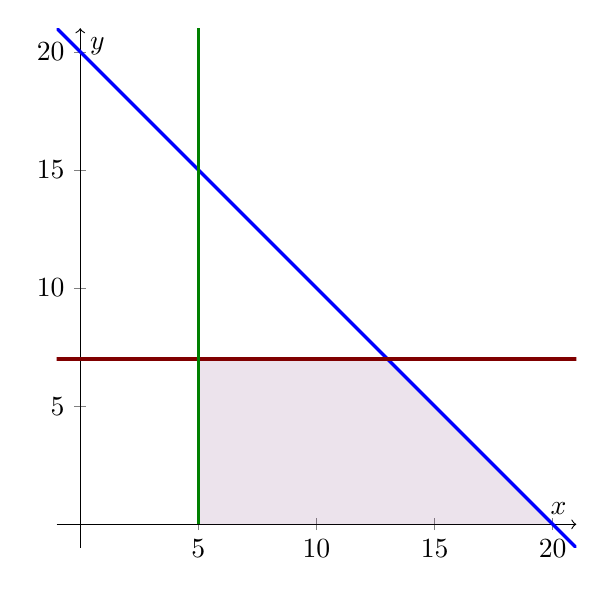
\begin{tikzpicture}
\begin{axis}[
    xmin=-1, xmax=21,
    ymin=-1, ymax=21,
    axis lines=center,
    axis on top=false,
    domain=0:1,
    x=0.3cm,
    y=0.3cm,
    xtick={0,5,...,20},
    xticklabels={0,5,...,20},
    ytick={0,5,...,20},
    yticklabels={0,5,...,20},
    axis lines=middle,
    axis line style={->},
    xlabel={$x$},
    ylabel={$y$},
    %grid=major
    ]
	\addplot [thick,color=blue,fill=blue!50!cyan!50!red, 
                    fill opacity=0.15,draw opacity=0]coordinates {
            (5, 0)
            (5,7)
            (13,7)
            (20,0) };   
	\addplot [very thick,blue,domain=-10:30] {-x+20};
	\addplot [very thick,red!50!black,domain=-10:30] {7};
	\addplot [very thick,green!50!black] coordinates{(5,0)(5,21)};
\end{axis}
\end{tikzpicture}
\end{center}
The shaded region is called the \emph{feasible region} because it represents all the combinations $(x,y)$ that are allowed by the constraints.  Any point outside that region, if we substituted it into the system of inequalities, would violate one or more of the constraints.  \marginnote{Note the \emph{unstated} non-negative constraint}Notice that we used a constraint that we never stated: $y$ must be positive, since Julie can't babysit fewer than 0 hours per week.

\begin{formula}{Feasible Region}
The feasible region in a linear programming problem is the set of all points that satisfy all the constraints.  The answer will be a point in the feasible region.
\end{formula}

We now know that the optimal solution will be somewhere in that shaded region, but there are still too many possibilities to check each one individually.  This is where the power of linear programming comes into play, with the following theorem.

\begin{proc}{Fundamental Theorem of Linear Programming (simple form)}
The optimal point(s) will lie either at the corner of the feasible region or along one of its edges.
\end{proc}

We'll come back a little bit later to think about why this makes sense, but for now we'll use it to answer the example we're working on.  Now, instead of having to check \emph{all} the points in the feasible region, we can simply check the four corners.

This is what makes linear programming so useful: we've turned an impossible problem into a simple one.  All we have to do is find the coordinates of the corner points and evaluate the objective function for each of those combinations of $x$ and $y$ to find the best possible one.\\

\paragraph{Find the Corner Points} Finding \marginnote{\bfseries Step 5}the corner points is equivalent to solving four systems of equations; each time we solve a system of equations, we find the point where two lines cross.
\begin{enumerate}
\item Find where $x+y=20$ and $y=7$ intersect.
\begin{align*}
x+y&=20\\
y&=7
\end{align*}
The second equation immediately tells us that the $y$-coordinate of the intersection is 7, and we can substitute that into the first equation to find that the $x$-coordinate must be 13.

\item Find where $x=5$ and $y=7$ intersect.

For this one, we don't even have to try; we're immediately told the coordinates of the intersection.

\item Find where $x=5$ and $y=0$ intersect.

Again, it is clear that this point is $(5,0)$.

\item Find where $x+y=20$ and $y=0$ intersect.

Knowing that $y=0$, $x$ must be 20.
\end{enumerate}

Thus, the corner points--sometimes called \emph{vertices}--are
\begin{center}
\marginnote{The corner points\\ (vertices)}$(13,7)$, $(5,7)$, $(5,0)$, and $(20,0)$
\end{center}

These are the only four candidates for the optimal point; Julie will earn the most money by using one of these combinations of the number of hours spent doing each job.  One of these combinations will also yield the \emph{least} possible money she could earn while still doing these jobs, but that's not the point we really want to find.\\
\vfill
\pagebreak

\paragraph{Evaluate the Objective Function at the Corners} Since \marginnote{\bfseries Step 6}we know that one of these four points is the optimal point, all we have to do is find what Julie's revenue would be if she worked each combination of hours.

Remember that the objective function (from Step 2) is \[r=8x+9.75y.\]  We evaluate this function at the four corner points, and we summarize our results in the table below.
\begin{center}
\begin{tabular}{|c c | c|}
\hline
$x$ & $y$ & $r=8x+9.75y$\\
\hline
& & \\
\rowcolor{green!30!white}13 & 7 & \marginnote{The optimal solution}172.25\\
5 & 7 & 108.25\\
5 & 0 & 40\\
20 & 0 & 160\\
\hline
\end{tabular}
\end{center}

The \marginnote{\bfseries Conclusion}optimal point is the row highlighted above: by walking the dog for 13 hours per week and babysitting for 7 hours per week, Julie will maximize her earnings.

This example illustrates the general process for solving linear programming problems: it all boils down to finding the few candidates for the optimal point (namely, the corners of the feasible region) and checking the objective function at each of these candidate points.

\begin{proc}{Solving Linear Programming Problems}
\begin{enumerate}
\item Identify the variables.  Look for the quantities in the problem for which you are asked to decide the value.
\item Find the objective function.  Define the quantity you are asked to maximize or minimize in terms of the variables.
\item Find the constraints.  Look in the problem statement for limitations, and then describe these in terms of the variables.  Note that in most problems, it'll be implied that the variables are nonnegative, but rarely stated.  Make sure to account for this.
\item Graph the feasible region.  Write the constraints as a system of linear inequalities, then graph the solution set for the system (the overlap of the individual solutions).
\item Find the corner points.  Solve as many systems of equations that you need to in order to find where all the constraint lines intersect.
\item Evaluate the objective function at the corners.  Plug the $x$- and $y$-coordinates of each of the corner points into the objective function.  The largest result will be the overall maximum, and the smallest result will be the overall minimum.
\end{enumerate}
\end{proc}
\vfill
\pagebreak

We'll illustrate two more examples in this section.

\begin{tcolorbox}[sharp corners=all]
\marginnote{\href{https://www.youtube.com/watch?v=xNaNT6pEih0}{\fontfamily{fvs}\selectfont \Large\color{black!70!blue!80!cyan}\uppercase{\bfseries\centering EXAMPLE \theExampleCounter}
}} Express Bike Shop offers custom bike kits.  The standard kit requires 15 hours of shop time, 8 hours of painting time, and 1 hour of inspection time.  The deluxe kit requires 12 hours of shop time, 12 hours of painting time, and 2 hours of inspection time.  Including all the employees, the bike shop has 120 hours available for shop time, 72 hours of painting time, and 11 hours of inspection time available each week.  How many customizations of each type should Express Bike Shop perform each week if each standard kit results in a profit of \$175 and the deluxe kits each result in a profit of \$275?  What is the maximum profit?
\end{tcolorbox}
\stepcounter{ExampleCounter}

\paragraph{Identify the Variables} Here \marginnote{\bfseries Step 1}we are asked how many customizations of each type to do, so these will be our variables.
\begin{align*}
x &= \textrm{ number of standard kits}\\
y &= \textrm{ number of deluxe kits}
\end{align*}

\paragraph{Find the Objective Function} The \marginnote{\bfseries Step 2}goal here is to maximize profit, so we need to define the profit function in terms of how many of each kit is sold.  The total profit is the profit that comes from each kind of kit, which is the number of kits times the profit per kit:
\[p=175x+275y\]

\paragraph{Find the Constraints} The \marginnote{\bfseries Step 3}limitations are the following:
\begin{itemize}
\item There are 120 hours of shop time, so we can use up to and including 120 hours between the two types of customizations.
\item There are 72 hours of painting time.
\item There are 11 hours of inspection time.
\item The number of kits must be 0 or greater.  This was never said, but it is clear that it must be true.
\end{itemize}
Writing the constraints in terms of the variables:
\begin{itemize}
\item The number of hours of shop time required is the sum of the number of hours required for each job times the number of jobs of that type.  This must be less than or equal to 120.
\[15x+12y \leq 120\]
\item Similarly, for painting time:
\[8x+12y \leq 72\]
\item Finally, for inspection time:
\[1x+2y \leq 11\]
\item The implied nonnegative constraints:
\begin{align*}
x &\geq 0\\
y &\geq 0
\end{align*}
\end{itemize}

Summarizing the constraints:
\begin{align*}
\color{blue}15x+12y &\color{blue}\leq 120\\
\color{green!50!black}8x+12y &\color{green!50!black}\leq 72\\
\color{red!50!black}x+2y &\color{red!50!black}\leq 11\\
x &\geq 0\\
y &\geq 0
\end{align*}
\vfill
\pagebreak

\paragraph{Graph the Feasible Region} The \marginnote{\bfseries Step 4}graph is shown below.  Notice that the nonnegative constraints simply mean that we'll be limited to the upper-right quadrant of the coordinate plane.  We graphed the lines using the intercepts, because then we have some of the corner points already labeled, saving us some time later.

\begin{center}
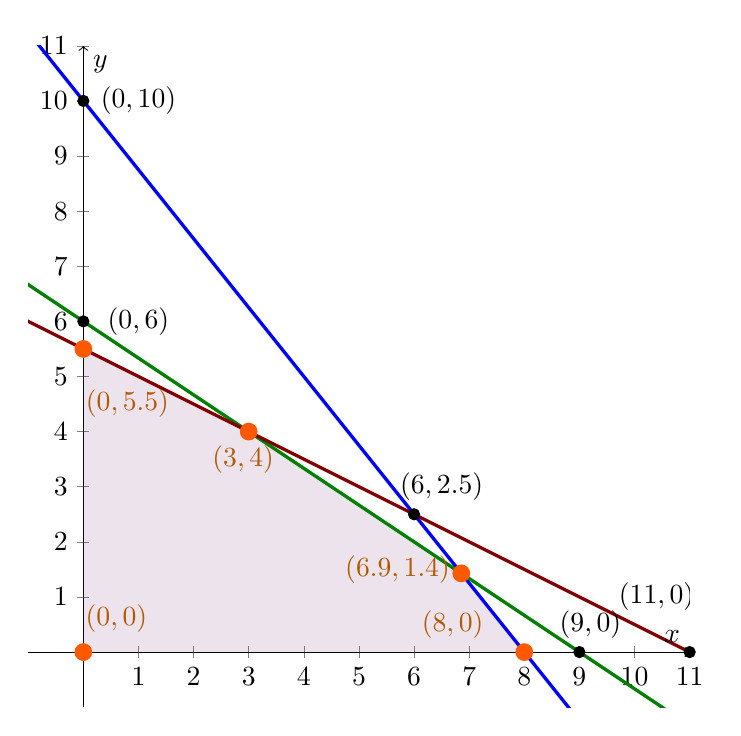
\begin{tikzpicture}
\begin{axis}[
    xmin=-1, xmax=11,
    ymin=-1, ymax=11,
    axis lines=center,
    axis on top=false,
    domain=0:1,
    x=0.7cm,
    y=0.7cm,
    xtick={0,1,...,20},
    xticklabels={0,1,...,20},
    ytick={0,1,...,20},
    yticklabels={0,1,...,20},
    axis lines=middle,
    axis line style={->},
    xlabel={$x$},
    ylabel={$y$},
    %grid=major
    ]
    \addplot [only marks,color=black] table {
	0 10
	0 6
	9 0
	11 0
	6 2.5
	};  
	\addplot [only marks,color=orange!70!red, mark size=3pt] table {
	0 5.5
	3 4
	8 0
	6.857 1.429
	0 0
	}; 
	\addplot [thick,color=blue,fill=blue!50!cyan!50!red, 
                    fill opacity=0.15,draw opacity=0]coordinates {
            (0,5.5)
            (3,4)
            (6.857, 1.429)
            (8,0)
            (0,0) };   
	\addplot [very thick,blue,domain=-10:30] {-(5/4)*x+10};
	\addplot [very thick,green!50!black,domain=-10:30] {-(2/3)*x+6};
	\addplot [very thick,red!50!black,domain=-10:30] {-(1/2)*x+5.5};
    \node (A) at (axis cs:1,10) {$(0,10)$};
    \node (B) at (axis cs:1,6) {$(0,6)$};
    \node (C) at (axis cs:0.8,4.5) {\color{orange!70!black} $(0,5.5)$};
    \node (D) at (axis cs:0.6,0.6) {\color{orange!70!black} $(0,0)$};
    \node (E) at (axis cs:6.7,0.5) {\color{orange!70!black} $(8,0)$};
    \node (F) at (axis cs:2.9,3.5) {\color{orange!70!black} $(3,4)$};
    \node (G) at (axis cs:5.7,1.5) {\color{orange!70!black} $(6.9,1.4)$};
    \node (H) at (axis cs:6.5,3) {$(6,2.5)$};
    \node (I) at (axis cs:9.2,0.5) {$(9,0)$};
    \node (J) at (axis cs:10.4,1) {$(11,0)$};
\end{axis}
\end{tikzpicture}
\end{center}

\paragraph{Find the Corner Points} By \marginnote{\bfseries Step 5}graphing using the intercepts, we found three of the corners along the way:
\begin{center}
$(0,0)$, $(0,5.5)$, and $(8,0)$
\end{center}
To find the other two (already shown on the graph above, along with all the other intersections that we don't need), we need to solve the following systems of equations:
\begin{center}
\begin{tabular}{c c}
{$\begin{aligned}
\color{green!50!black}8x+12y &\color{green!50!black}= 72\\
\color{red!50!black}x+2y &\color{red!50!black}= 11
\end{aligned}$} \hspace*{0.75in}
& 
{$\begin{aligned}
\color{blue}15x+12y &\color{blue}= 120\\
\color{green!50!black}8x+12y &\color{green!50!black}= 72
\end{aligned}$}\\
& \\
Solution: $(3,4)$ \hspace*{0.75in} & Solution: $\left(\dfrac{48}{7},\dfrac{10}{7}\right)$
\end{tabular}
\end{center}

We don't show the process of solving these systems of equations, but they can be done using either substitution or elimination (or graphing with a calculator).

Thus, the five vertices are
\begin{center} 
$(0,0)$, $(0,5.5)$, $(3,4)$, $\left(\dfrac{48}{7},\dfrac{10}{7}\right)$, and $(8,0)$
\end{center}

\paragraph{Evaluate the Objective Function at the Corners} If \marginnote{\bfseries Step 6}we evaluate the objective function from Step 2 at each of these vertices, we get the results summarized in the table below.
\begin{center}
\begin{tabular}{|c c | c|}
\hline
$x$ & $y$ & $p=175x+275y$\\
\hline
& & \\
0 & 0 & 0\\
0 & 5.5 & 1512.5\\
\rowcolor{green!30!white}3 & 4 & 1625\\
48/7 & 10/7 & 1592.86\\
8 & 0 & 1400\\
\hline
\end{tabular}
\end{center}

The \marginnote{\bfseries Conclusion}optimal point is the row highlighted above: by selling 3 standard kits and 4 deluxe kits per week, the bike shop will maximize their profits.  This maximum profit is \$1625 per week.
\vfill
\pagebreak

\subsection{Why the Fundamental Theorem Works}
We've used the theorem for each of the last two examples, accepting that the optimal value occurs at one of the corners (or along an edge, but neither example had that occur).  But now we'd like to see why the theorem is true.  We won't give a detailed proof, but we can make a convincing graphical argument.

Suppose we have the feasible region from the first example.
\begin{center}
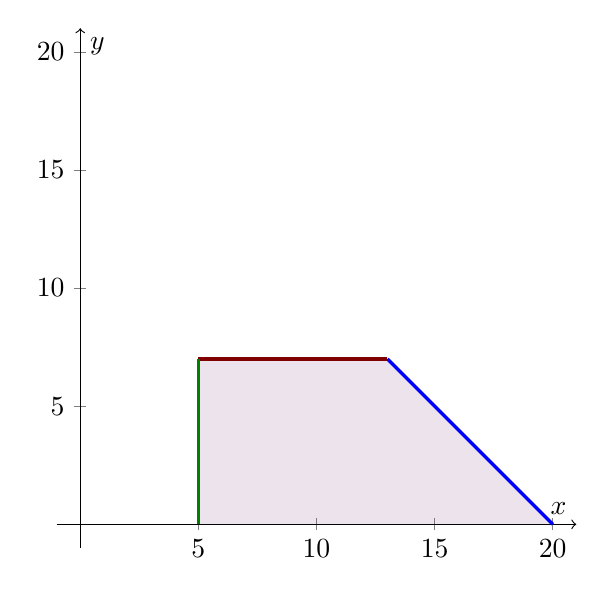
\begin{tikzpicture}
\begin{axis}[
    xmin=-1, xmax=21,
    ymin=-1, ymax=21,
    axis lines=center,
    axis on top=false,
    domain=0:1,
    x=0.3cm,
    y=0.3cm,
    xtick={0,5,...,20},
    xticklabels={0,5,...,20},
    ytick={0,5,...,20},
    yticklabels={0,5,...,20},
    axis lines=middle,
    axis line style={->},
    xlabel={$x$},
    ylabel={$y$},
    %grid=major
    ]
	\addplot [thick,color=blue,fill=blue!50!cyan!50!red, 
                    fill opacity=0.15,draw opacity=0]coordinates {
            (5, 0)
            (5,7)
            (13,7)
            (20,0) };   
	\addplot [very thick,blue,domain=13:20] {-x+20};
	\addplot [very thick,red!50!black,domain=5:13] {7};
	\addplot [very thick,green!50!black] coordinates{(5,0)(5,7)};
\end{axis}
\end{tikzpicture}
\end{center}

Recall that the objective function in that example was $r=8x+9.75y$.  Now we ask: could Julie make \$200?  In that case, $200=8x+9.75y$, which is a linear equation.  If we graph it, it will show all the combinations of $x$ and $y$ (the number of hours spent at each job) for which she makes \$200.

However, notice that these points all lie outside the feasible region, which means that Julie cannot make \$200 and still satisfy all the constraints.

Okay, but what about \$150?  Now the objective function becomes $150=8x+9.75$, and we can graph that as well.

\begin{center}
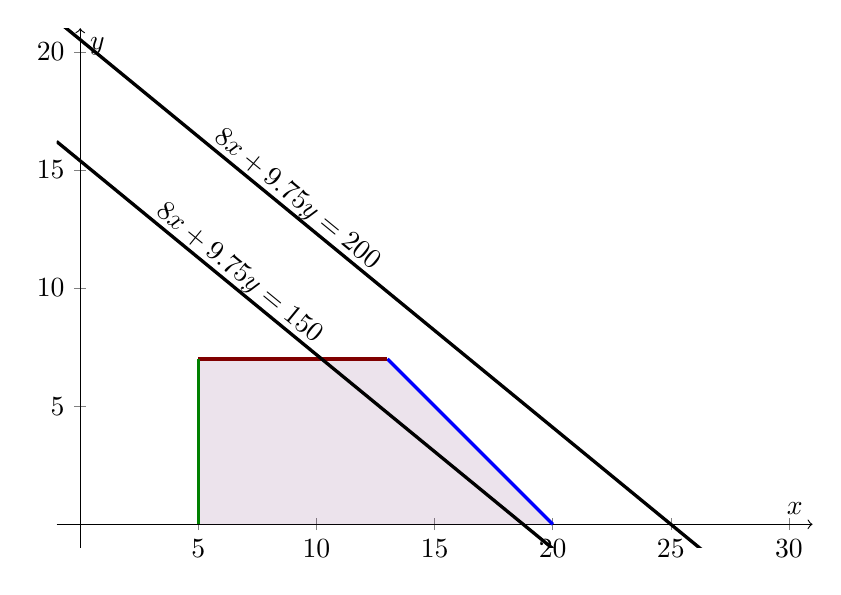
\begin{tikzpicture}
\begin{axis}[
    xmin=-1, xmax=31,
    ymin=-1, ymax=21,
    axis lines=center,
    axis on top=false,
    domain=0:1,
    x=0.3cm,
    y=0.3cm,
    xtick={0,5,...,30},
    xticklabels={0,5,...,30},
    ytick={0,5,...,20},
    yticklabels={0,5,...,20},
    axis lines=middle,
    axis line style={->},
    xlabel={$x$},
    ylabel={$y$},
    %grid=major
    ]
	\addplot [thick,color=blue,fill=blue!50!cyan!50!red, 
                    fill opacity=0.15,draw opacity=0]coordinates {
            (5, 0)
            (5,7)
            (13,7)
            (20,0) };   
	\addplot [very thick,blue,domain=13:20] {-x+20};
	\addplot [very thick,red!50!black,domain=5:13] {7};
	\addplot [very thick,domain=-1:27] {-(8/9.75)*x+200/9.75} node [above,sloped,pos=0.35,inner sep=0pt] {$8x+9.75y=200$};
	\addplot [very thick,domain=-1:20] {-(8/9.75)*x+150/9.75} node [above,sloped,pos=0.35,inner sep=0pt] {$8x+9.75y=150$};
	\addplot [very thick,green!50!black] coordinates{(5,0)(5,7)};
\end{axis}
\end{tikzpicture}
\end{center}

Immediately, we notice two things:
\begin{enumerate}
\item The second line cuts through the feasible region, meaning that there \emph{are} cases where Julie can make \$150 and satisfy all the constraints.
\item The two lines are parallel.  If we drew a third line with a third value for Julie's revenue, it would also be parallel to these two, because the coefficients of $x$ and $y$, which determine the slope, would not change.  These parallel lines are called \emph{level curves}, and changing the value of the revenue simply slides these level curves in and out.
\end{enumerate}

\begin{center}
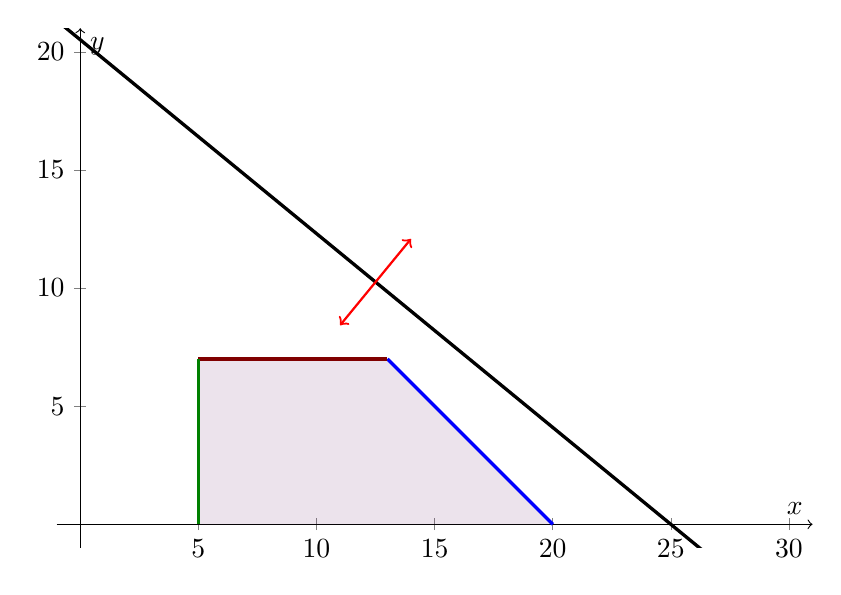
\begin{tikzpicture}
\begin{axis}[
    xmin=-1, xmax=31,
    ymin=-1, ymax=21,
    axis lines=center,
    axis on top=false,
    domain=0:1,
    x=0.3cm,
    y=0.3cm,
    xtick={0,5,...,30},
    xticklabels={0,5,...,30},
    ytick={0,5,...,20},
    yticklabels={0,5,...,20},
    axis lines=middle,
    axis line style={->},
    xlabel={$x$},
    ylabel={$y$},
    %grid=major
    ]
	\addplot [thick,color=blue,fill=blue!50!cyan!50!red, 
                    fill opacity=0.15,draw opacity=0]coordinates {
            (5, 0)
            (5,7)
            (13,7)
            (20,0) };   
	\addplot [very thick,blue,domain=13:20] {-x+20};
	\addplot [very thick,red!50!black,domain=5:13] {7};
	\addplot [very thick,domain=-1:27] {-(8/9.75)*x+200/9.75};
	\addplot [thick,red,style=->,domain=12.5:14] {(9.75/8)*x-4.98};
	\addplot [thick,red,style=<-,domain=11:12.5] {(9.75/8)*x-4.98};
	\addplot [very thick,green!50!black] coordinates{(5,0)(5,7)};
\end{axis}
\end{tikzpicture}\\
{\footnotesize Changing the value of the objective function slides the level curve in and out}
\end{center}

So it's impossible to make \$200, given the constraints, but it's possible to make \$150.  However, notice that we could slide the \$150 line out a little bit before getting out of the feasible region, so \$150 is not the \emph{best} that we can do.

In general, if we start with a value for the objective function that is too high to be possible, as we start to lower it we find that it will first hit the feasible region either at a corner or along an edge.
\begin{center}
\begin{tabular}{c c}
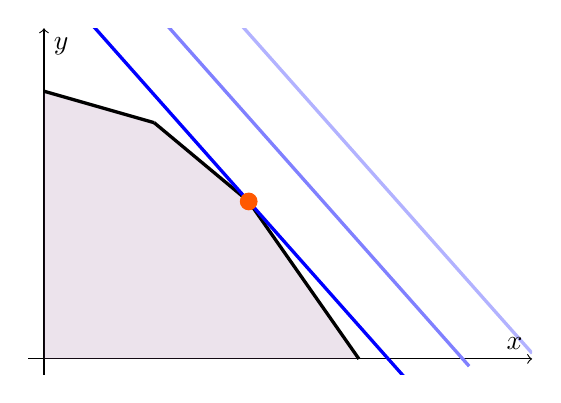
\begin{tikzpicture}
\begin{axis}[
    xmin=-1, xmax=31,
    ymin=-1, ymax=21,
    axis lines=center,
    axis on top=false,
    domain=0:1,
    x=0.2cm,
    y=0.2cm,
    xtick={-10,50,...,110},
    xticklabels={},
    ytick={-10,50,...,110},
    yticklabels={},
    axis lines=middle,
    axis line style={->},
    xlabel={$x$},
    ylabel={$y$},
    %grid=major
    ]
    \addplot [only marks,color=orange!70!red, mark size=3pt] table {
	13 10
	}; 
	\addplot [thick,color=blue,fill=blue!50!cyan!50!red, 
                    fill opacity=0.15,draw opacity=0]coordinates {
            (0, 0)
            (0,17)
            (7,15)
            (13,10)
            (20,0) };   
	\addplot [very thick,domain=0:7] {-(2/7)*x+17};
	\addplot [very thick,domain=7:13] {-(5/6)*x+125/6};
	\addplot [very thick,domain=13:20] {-(10/7)*x+200/7};
	\addplot [very thick,blue!30!white,domain=-1:31] {-(11/9.75)*x+106/3};
	\addplot [very thick,blue!50!white,domain=-1:27] {-(11/9.75)*x+90/3};
	\addplot [very thick,blue,domain=-1:27] {-(11/9.75)*x+74/3};
\end{axis}
\end{tikzpicture}
&
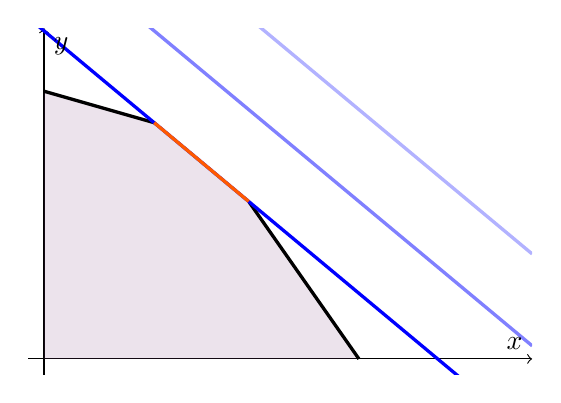
\begin{tikzpicture}
\begin{axis}[
    xmin=-1, xmax=31,
    ymin=-1, ymax=21,
    axis lines=center,
    axis on top=false,
    domain=0:1,
    x=0.2cm,
    y=0.2cm,
    xtick={-10,50,...,110},
    xticklabels={},
    ytick={-10,50,...,110},
    yticklabels={},
    axis lines=middle,
    axis line style={->},
    xlabel={$x$},
    ylabel={$y$},
    %grid=major
    ]
	\addplot [thick,color=blue,fill=blue!50!cyan!50!red, 
                    fill opacity=0.15,draw opacity=0]coordinates {
            (0, 0)
            (0,17)
            (7,15)
            (13,10)
            (20,0) };   
	\addplot [very thick,domain=0:7] {-(2/7)*x+17};
	\addplot [very thick,domain=13:20] {-(10/7)*x+200/7};
	\addplot [very thick,blue!30!white,domain=-1:31] {-(5/6)*x+195/6};
	\addplot [very thick,blue!50!white,domain=-1:31] {-(5/6)*x+160/6};
	\addplot [very thick,blue,domain=-1:27] {-(5/6)*x+125/6};
	
	\addplot [very thick,orange!70!red,domain=7:13] {-(5/6)*x+125/6};
\end{axis}
\end{tikzpicture}\\
{\footnotesize Optimal point at a corner} & {\footnotesize Optimal points along an edge}
\end{tabular}
\end{center}

We haven't done any examples where the optimal points lie along an edge, but the principle remains the same.  If two of the corner points have the same value for the objective function, then the optimal points are all the points on the edge that connects those two corners.  In that case, the choice of any point along that edge will be an acceptable position to be in.
\vfill
\pagebreak

\begin{center}
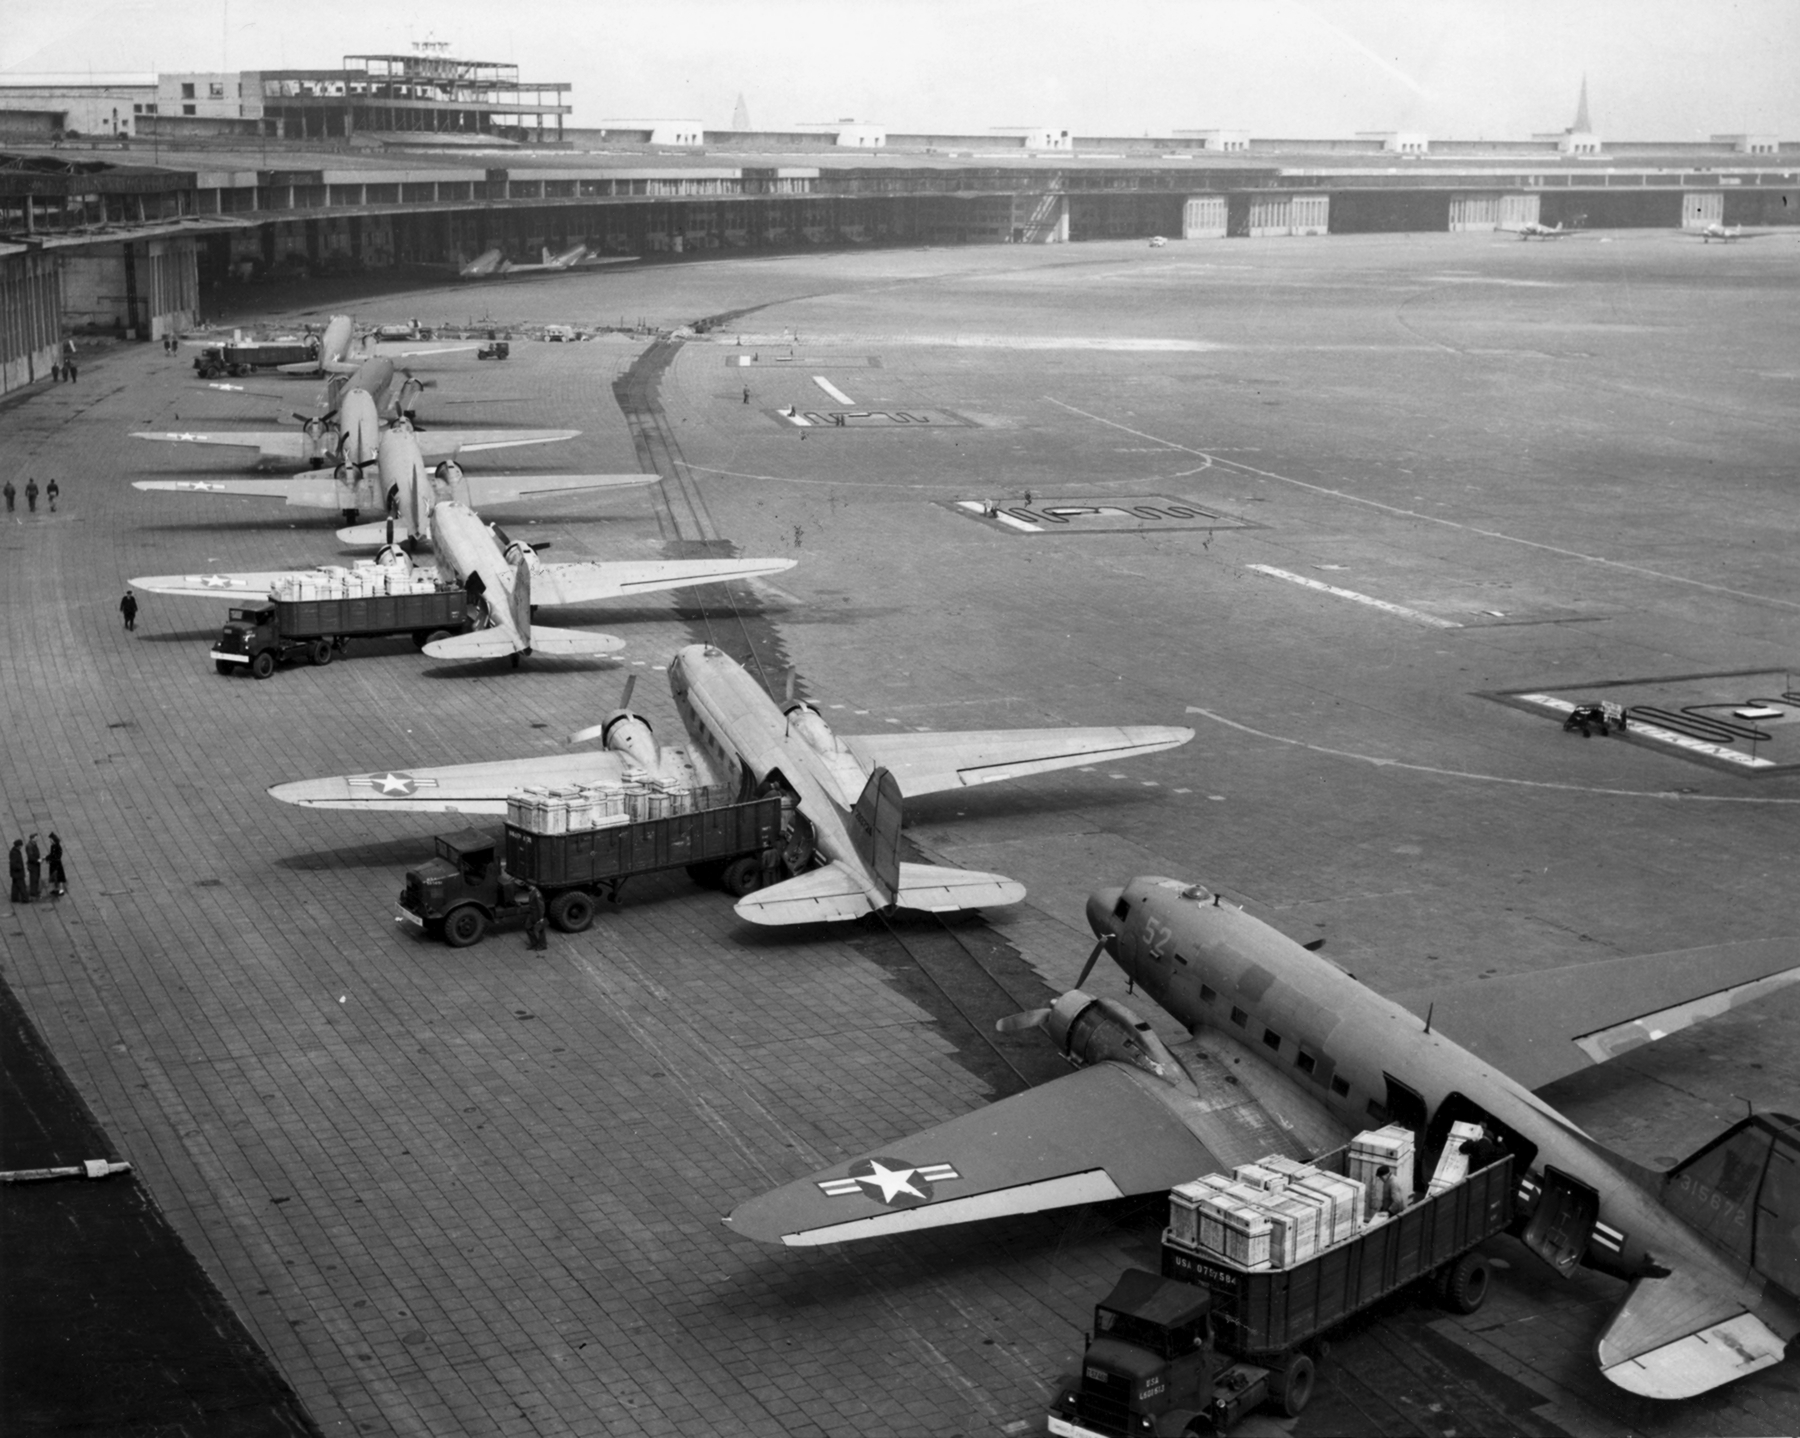
\includegraphics[width=0.6\textwidth]{BerlinAirlift2}
\end{center}

\begin{tcolorbox}[sharp corners=all]
\marginnote{\href{https://www.youtube.com/watch?v=TuT37Ar9diw}{\fontfamily{fvs}\selectfont \Large\color{black!70!blue!80!cyan}\uppercase{\bfseries\centering EXAMPLE \theExampleCounter}
}} Here is a \emph{very} simplified version of the problem facing the planners of the Berlin Airlift (in reality there were over fifty variables to consider, rather than just two).\\

The goal is to maximize the weekly cargo capacity of American and British planes flying into Berlin.  The cargo capacity of an American plane is 30,000 cubic feet and the cargo capacity of a British plane is 20,000 cubic feet.  However, there are only enough runways to allow 56 flights per week, plus the total cost per week is limited to \$300,000 (an American flight costs \$9000 and a British flight costs \$5000).  Finally, only 512 crew members are available; each American flight requires 16 crew members and each British flight requires 8.  How many American and British planes should be used to maximize the cargo capacity?
\end{tcolorbox}

\paragraph{Identify the Variables} Our \marginnote{\bfseries Step 1}job is to decide how many of each type of plane to use.
\begin{align*}
x &= \textrm{ number of American planes}\\
y &= \textrm{ number of British planes}
\end{align*}

\paragraph{Find the Objective Function} The \marginnote{\bfseries Step 2}goal here is to maximize cargo, so we look at how much cargo each type of plane can carry.
\[c=30,000x+20,000y\]

\paragraph{Find the Constraints} The \marginnote{\bfseries Step 3}limitations are the following:
\begin{itemize}
\item Only 56 flights total are allowed.
\[x+y \leq 56\]
\item The total cost cannot exceed \$300,000.
\[9000x+5000y \leq 300,000\]
\item Only 512 crew members are available.
\[16x+8y \leq 512\]
\item As usual, it isn't stated, but it only makes sense if $x$ and $y$ are both nonnegative.
\begin{align*}
x &\geq 0\\
y &\geq 0
\end{align*}
\end{itemize}

Summarizing the constraints:
\begin{align*}
\color{blue}x+y &\color{blue}\leq 56\\
\color{green!50!black}9000x+5000y &\color{green!50!black}\leq 300,000\\
\color{red!50!black}16x+8y &\color{red!50!black}\leq 512\\
x &\geq 0\\
y &\geq 0
\end{align*}

\paragraph{Graph the Feasible Region} The \marginnote{\bfseries Step 4}graph is shown below.  

\begin{center}
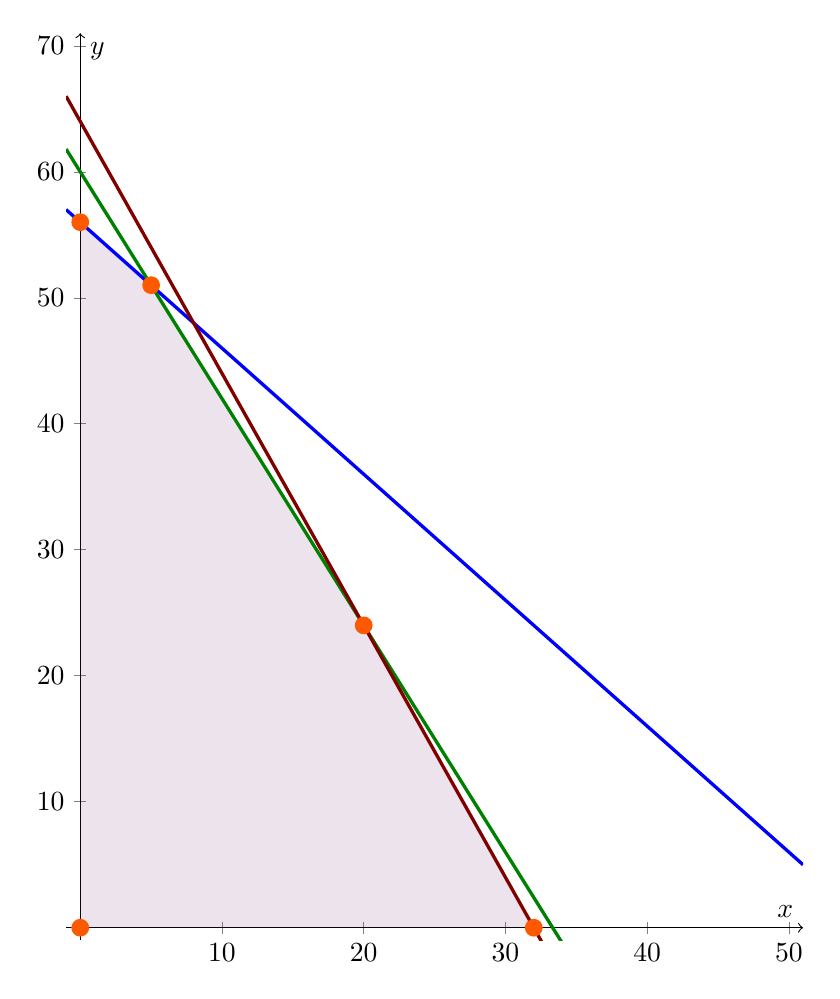
\begin{tikzpicture}
\begin{axis}[
    xmin=-1, xmax=51,
    ymin=-1, ymax=71,
    axis lines=center,
    axis on top=false,
    domain=0:1,
    x=0.18cm,
    y=0.16cm,
    xtick={0,10,...,60},
    xticklabels={0,10,...,60},
    ytick={0,10,...,80},
    yticklabels={0,10,...,80},
    axis lines=middle,
    axis line style={->},
    xlabel={$x$},
    ylabel={$y$},
    %grid=major
    ]
	\addplot [only marks,color=orange!70!red, mark size=3pt] table {
	0 56
	5 51
	20 24
	32 0
	0 0
	}; 
	\addplot [thick,color=blue,fill=blue!50!cyan!50!red, 
                    fill opacity=0.15,draw opacity=0]coordinates {
            (0,0)
            (0,56)
            (5, 51)
            (20,24)
            (32,0) };   
	\addplot [very thick,blue,domain=-1:51] {-x+56};
	\addplot [very thick,green!50!black,domain=-1:51] {-(9/5)*x+60};
	\addplot [very thick,red!50!black,domain=-1:51] {-2*x+64};
\end{axis}
\end{tikzpicture}
\end{center}

\paragraph{Find the Corner Points} By \marginnote{\bfseries Step 5}graphing using the intercepts, we found three of the corners along the way:
\begin{center}
$(0,0)$, $(0,56)$, and $(32,0)$
\end{center}
To find the other two, we need to solve the following systems of equations:
\begin{center}
\begin{tabular}{c c}
{$\begin{aligned}
\color{green!50!black}9000x+5000y &\color{green!50!black}= 300,000\\
\color{red!50!black}16x+8y &\color{red!50!black}= 512
\end{aligned}$} \hspace*{0.75in}
& 
{$\begin{aligned}
\color{blue}x+y &\color{blue}= 56\\
\color{green!50!black}9000x+5000y &\color{green!50!black}= 300,000
\end{aligned}$}\\
& \\
Solution: $(20,24)$ \hspace*{0.75in} & Solution: $(5,51)$
\end{tabular}
\end{center}

Again, for sake of space, we don't show the process of solving these systems of equations, but they can be done using either substitution or elimination (or graphing with a calculator).

Thus, the five vertices are
\begin{center} 
$(0,0)$, $(0,56)$, $(5,51)$, $(20,24)$, and $(32,0)$
\end{center}

\paragraph{Evaluate the Objective Function at the Corners} If \marginnote{\bfseries Step 6}we evaluate the objective function from Step 2 at each of these vertices, we get the results summarized in the table below.
\begin{center}
\begin{tabular}{|c c | c|}
\hline
$x$ & $y$ & $c=30,000x+20,000y$\\
\hline
& & \\
0 & 0 & 0\\
0 & 56 & 1,120,000\\
\rowcolor{green!30!white}5 & 51 & 1,170,000\\
20 & 24 & 1,080,000\\
32 & 0 & 960,000\\
\hline
\end{tabular}
\end{center}

The \marginnote{\bfseries Conclusion}optimal point is the row highlighted above: by using 5 American planes and 51 British planes, the Allies will maximize the cargo flying into Berlin.  The maximum cargo that can be carried under these conditions is 1,170,000 cubic feet per week.

\begin{exercises}
\textit{In exercises 1--4, write an objective function for the given situation in terms of the variables defined.}

\ptwo{A fence company sells wooden and metal fences.  Let $x$ represent the number of wooden fences they sell and let $y$ represent the number of metal fences.  They make a profit of \$320 for each wooden fence and \$280 for each metal fence.
}
\ptwo{You are placing mulch in your yard, and you find that pine chips cost \$2 per bag, while oak chips cost \$4 per bag.  You want to minimize total cost.  Let $x$ be the number of bags of pine chips and $y$ be the number of bags of oak chips.
}

\ptwo{An auto repair shop offers tire rotations and oil changes.  They make a profit of \$25 on each oil change and a profit of \$18 on each tire rotation.  Let $x$ be the number of oil changes and $y$ be the number of tire rotations.
}
\ptwo{Taking a pill of Medicine A gives you 6 mg of an undesired substance, and Medicine B gives you 8 mg of the undesired substance (you want to minimize the amount of this substance).  Let $x$ be the number of A pills you take and $y$ be the number of B pills you take.
}

\textit{In exercises 5--8, write an inequality to represent each constraint given.}

\ptwo{Manufacturing one chair ($x$) requires 6 ft of aluminum tube, and manufacturing one table ($y$) requires 12 ft of aluminum tube.  There are 500 ft of aluminum tube available.
}
\ptwo{Each oil change ($x$) takes 20 minutes and each tire rotation ($y$) takes 15 minutes.  There are a total of 2400 minutes available.
}

\ptwo{You must take at least 3 pills of Medicine A ($x$) and at least 2 pills of Medicine B ($y$).
}
\ptwo{Mowing a large yard ($x$) uses 0.25 gallons of gasoline, and mowing a small yard ($y$) uses 0.1 gallons of gasoline.  There are 5 gallons of gasoline available.
}

\textit{In exercises 9--12, graph each feasible region and list the corner points.}

\ptwo{Feasible region:
\begin{align*}
2x+4y &\leq 20\\
4x+2y &\leq 16\\
x &\geq 0\\
y &\geq 0
\end{align*}
\begin{center}
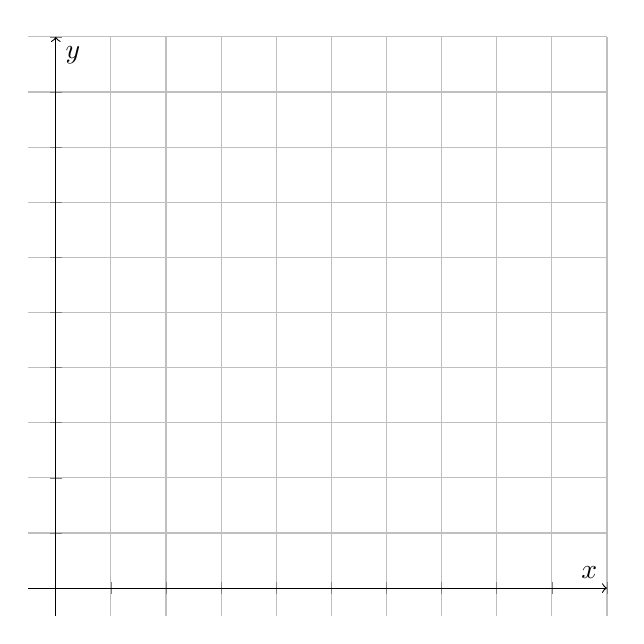
\begin{tikzpicture}
\begin{axis}[
    xmin=-0.5, xmax=10,
    ymin=-0.5, ymax=10,
    axis lines=center,
    axis on top=false,
    domain=0:1,
    x=0.7cm,
    y=0.7cm,
    xtick={0,1,...,10},
    xticklabels={},
    ytick={0,1,...,10},
    yticklabels={},
    axis lines=middle,
    axis line style={->},
    xlabel={$x$},
    ylabel={$y$},
    grid=major
    ]
\end{axis}
\end{tikzpicture}
\end{center}
}
\ptwo{Feasible region:
\begin{align*}
20x+40y &\leq 160\\
18x+9y &\leq 90\\
x &\geq 0\\
y &\geq 0
\end{align*}
\begin{center}
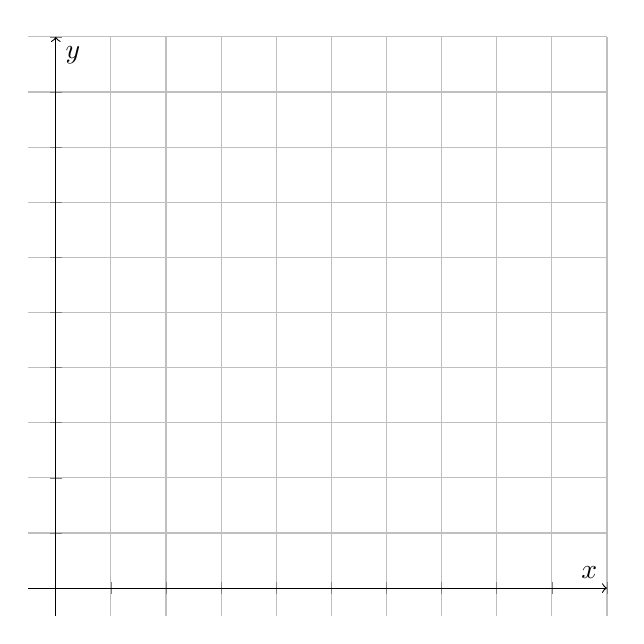
\begin{tikzpicture}
\begin{axis}[
    xmin=-0.5, xmax=10,
    ymin=-0.5, ymax=10,
    axis lines=center,
    axis on top=false,
    domain=0:1,
    x=0.7cm,
    y=0.7cm,
    xtick={0,1,...,10},
    xticklabels={},
    ytick={0,1,...,10},
    yticklabels={},
    axis lines=middle,
    axis line style={->},
    xlabel={$x$},
    ylabel={$y$},
    grid=major
    ]
\end{axis}
\end{tikzpicture}
\end{center}
}

\ptwo{Feasible region:
\begin{align*}
2x+y &\leq 8\\
x+3y &\leq 6\\
x &\geq 0\\
y &\geq 0
\end{align*}
\begin{center}
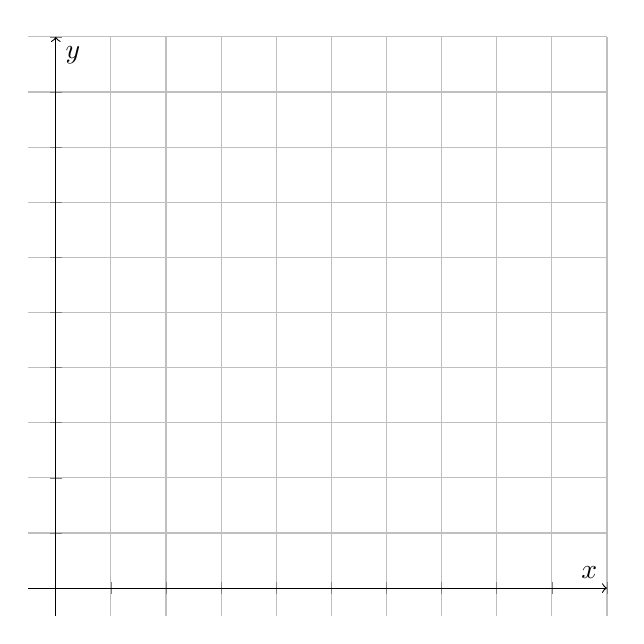
\begin{tikzpicture}
\begin{axis}[
    xmin=-0.5, xmax=10,
    ymin=-0.5, ymax=10,
    axis lines=center,
    axis on top=false,
    domain=0:1,
    x=0.7cm,
    y=0.7cm,
    xtick={0,1,...,10},
    xticklabels={},
    ytick={0,1,...,10},
    yticklabels={},
    axis lines=middle,
    axis line style={->},
    xlabel={$x$},
    ylabel={$y$},
    grid=major
    ]
\end{axis}
\end{tikzpicture}
\end{center}
}
\ptwo{Feasible region:
\begin{align*}
15x+5y &\leq 75\\
9x+9y &\leq 81\\
x &\geq 0\\
y &\geq 0
\end{align*}
\begin{center}
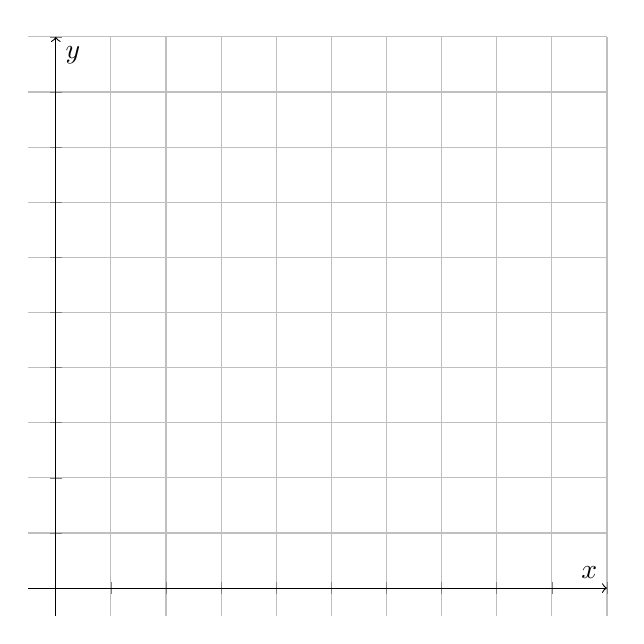
\begin{tikzpicture}
\begin{axis}[
    xmin=-0.5, xmax=10,
    ymin=-0.5, ymax=10,
    axis lines=center,
    axis on top=false,
    domain=0:1,
    x=0.7cm,
    y=0.7cm,
    xtick={0,1,...,10},
    xticklabels={},
    ytick={0,1,...,10},
    yticklabels={},
    axis lines=middle,
    axis line style={->},
    xlabel={$x$},
    ylabel={$y$},
    grid=major
    ]
\end{axis}
\end{tikzpicture}
\end{center}
}

\textit{In exercises 13--16, pick which of the given corner points maximizes the given objective function.}

\ptwo{Objective function: \[p=5x+7y\]
\hspace{0.25in} Corners: \[(0,0),\ (8,4),\ (6,5),\ (0,8),\ \textrm{and } (12,0)\]
}
\ptwo{Objective function: \[p=20x+12y\]
\hspace{0.25in} Corners: \[(18,9),\ (20,0),\ (0,36),\ \textrm{and } (12,10)\]
}

\ptwo{Objective function: \[p=95x+72y\]
\hspace{0.25in} Corners: \[(0,0),\ (5,7),\ (3,9),\ (0,10),\ \textrm{and } (7,0)\]
}
\ptwo{Objective function: \[p=28x+32y\]
\hspace{0.25in} Corners: \[(0,0),\ (12,9),\ (9,15),\ (0,13),\ \textrm{and } (15,0)\]
}

\pone{A graphic designer can design a magazine cover or a logo.  Her company makes a profit of \$800 for each magazine cover and \$500 for each logo.  She estimates that it takes her 4 hours of brainstorming for a magazine cover and 2 hours of brainstorming for a logo.  She'd like to keep the total brainstorming time under 24 hours a week.  Further, she estimates that it takes her 2 hours to lay out a magazine cover and 0.5 hours to sketch up a logo, and she must fit this into 10 hours a week.  Her boss requires her to design no more than 4 logos for each magazine cover she designs.  How many of each should she design in order to maximize the company's profits?  What is the maximum profit?
}

\pone{A manufacturer of ski clothing makes ski pants and ski jackets.  The profit on a pair of ski pants is \$2.00 and the profit on a jacket is \$1.50.  Both pants and jackets require the work of sewing operators and cutters.  There are 60 minutes of sewing operator time and 48 minutes of cutter time available.  It takes 8 minutes to sew one pair of ski pants and 4 minutes to sew one jacket.  Cutters take 4 minutes on pants and 8 minutes on a jacket.  Find the maximum profit and the number of pants and jackets the manufacturer should make in order to maximize the profit.
}

\pone{An automotive plant makes the Quartz and the Pacer.  The plant has a maximum production capacity of 1200 cars per week, and they can make at most 600 Quartz cars and 800 Pacers each week.  If the profit on a Quartz is \$500 and the profit on a Pacer is \$800, find how many of each type of car the plant should produce.  What is the maximum profit?
}

\pone{A farmer has a field of 70 acres in which he plants potatoes and corn.  The seed for potatoes costs \$20/acre, the seed for corn costs \$60/acre, and the farmer has set aside \$3000 to spend on seed.  The profit per acre of potatoes is \$150 and the profit for corn is \$50 an acre.  How many acres of each should the farmer plant?  What is the maximum profit?
}

\pone{A manufacturer produces two models of mountain bikes.  The times (in hours) required for assembling and painting each model are given by the following table:
\begin{center}
\begin{tabular}{|l|c|c|}
\hline
& Model A & Model B\\
\hline
Assembling & 5 & 4\\
\hline
Painting & 2 & 3\\
\hline
\end{tabular}
\end{center}
The maximum total weekly hours available in the assembly department and the painting department are 200 hours and 108 hours, respectively.  The profits per unit are \$25 for Model A and \$15 for Model B.  How many of each type should be produced to maximize profit?  What is the maximum profit?
}

\pone{A student earns \$10 per hour for tutoring and \$7 per hour as a teacher's aide.  To have enough free time for studies, he can work no more than 20 hours per week.  The tutoring center requires that each tutor spends at least three hours per week tutoring, but no more than eight hours per week.  How many hours should he work to maximize his earnings?  What are the maximum earnings?
}
\end{exercises}